\documentclass{article}
\usepackage{hyperref}
\usepackage[table,xcdraw]{xcolor}
\usepackage{xcolor}
\usepackage{graphicx}
\usepackage{lscape}
\usepackage[francais]{babel}
\usepackage[utf8]{inputenc}
\usepackage{verbatim}
\begin{document}
\title{Rapport de projet Picross}
\author{CONNES Victor \and PRYSIAZHNIUK Anastasiia \and BENAIS-HUGOT Charles \and RIVIERE Cecilie}
\maketitle
\tableofcontents 
\newpage
\section{Description du problème}

Le Picross est un casse-tête qui consiste à retrouver une figure depuis les indices. La figure à découvrir est une grille dans laquelle chaque case est de couleur noire ou blanche. Pour chacune des lignes et colonnes on dispose d'un indice qui est une séquence de nombres représentant les longueurs des blocs de cases noires contigũes de la ligne/colonne. Les blocs de cases noires sont séparés par au moins une case blanche.

\begin{table}[h]
\centering
\begin{tabular}{ccccccc}
\textbf{}  & \textbf{}                       & \textbf{3}                     & \textbf{4}                     & \textbf{4}                     & \textbf{4}                     & \textbf{3}                     \\ \cline{3-7} 
\textbf{2} & \multicolumn{1}{c|}{\textbf{2}} & \multicolumn{1}{c|}{\textbf{}} & \multicolumn{1}{c|}{\textbf{}} & \multicolumn{1}{c|}{\textbf{}} & \multicolumn{1}{c|}{\textbf{}} & \multicolumn{1}{c|}{\textbf{}} \\ \cline{3-7} 
\textbf{}  & \multicolumn{1}{c|}{\textbf{5}} & \multicolumn{1}{c|}{\textbf{}} & \multicolumn{1}{c|}{\textbf{}} & \multicolumn{1}{c|}{\textbf{}} & \multicolumn{1}{c|}{\textbf{}} & \multicolumn{1}{c|}{\textbf{}} \\ \cline{3-7} 
\textbf{}  & \multicolumn{1}{c|}{\textbf{5}} & \multicolumn{1}{c|}{\textbf{}} & \multicolumn{1}{c|}{\textbf{}} & \multicolumn{1}{c|}{\textbf{}} & \multicolumn{1}{c|}{\textbf{}} & \multicolumn{1}{c|}{\textbf{}} \\ \cline{3-7} 
\textbf{}  & \multicolumn{1}{c|}{\textbf{3}} & \multicolumn{1}{c|}{\textbf{}} & \multicolumn{1}{c|}{\textbf{}} & \multicolumn{1}{c|}{\textbf{}} & \multicolumn{1}{c|}{\textbf{}} & \multicolumn{1}{c|}{\textbf{}} \\ \cline{3-7} 
\textbf{}  & \multicolumn{1}{c|}{\textbf{1}} & \multicolumn{1}{c|}{\textbf{}} & \multicolumn{1}{c|}{\textbf{}} & \multicolumn{1}{c|}{\textbf{}} & \multicolumn{1}{c|}{\textbf{}} & \multicolumn{1}{c|}{\textbf{}} \\ \cline{3-7} 
\end{tabular}
\end{table}

\begin{table}[h]
\centering
\begin{tabular}{ccccccc}
\textbf{}  & \textbf{}                       & \textbf{3}                                                                    & \textbf{4}                                                                    & \textbf{4}                                                                    & \textbf{4}                                                                    & \textbf{3}                                                                    \\ \cline{3-7} 
\textbf{2} & \multicolumn{1}{c|}{\textbf{2}} & \multicolumn{1}{c|}{\cellcolor[HTML]{000000}{\color[HTML]{000000} \textbf{}}} & \multicolumn{1}{c|}{\cellcolor[HTML]{000000}\textbf{}}                        & \multicolumn{1}{c|}{\textbf{}}                                                & \multicolumn{1}{c|}{\cellcolor[HTML]{000000}\textbf{}}                        & \multicolumn{1}{c|}{\cellcolor[HTML]{000000}\textbf{}}                        \\ \cline{3-7} 
\textbf{}  & \multicolumn{1}{c|}{\textbf{5}} & \multicolumn{1}{c|}{\cellcolor[HTML]{000000}\textbf{}}                        & \multicolumn{1}{c|}{\cellcolor[HTML]{000000}\textbf{}}                        & \multicolumn{1}{c|}{\cellcolor[HTML]{000000}\textbf{}}                        & \multicolumn{1}{c|}{\cellcolor[HTML]{000000}\textbf{}}                        & \multicolumn{1}{c|}{\cellcolor[HTML]{000000}\textbf{}}                        \\ \cline{3-7} 
\textbf{}  & \multicolumn{1}{c|}{\textbf{5}} & \multicolumn{1}{c|}{\cellcolor[HTML]{000000}{\color[HTML]{000000} \textbf{}}} & \multicolumn{1}{c|}{\cellcolor[HTML]{000000}{\color[HTML]{000000} \textbf{}}} & \multicolumn{1}{c|}{\cellcolor[HTML]{000000}{\color[HTML]{000000} \textbf{}}} & \multicolumn{1}{c|}{\cellcolor[HTML]{000000}{\color[HTML]{000000} \textbf{}}} & \multicolumn{1}{c|}{\cellcolor[HTML]{000000}{\color[HTML]{000000} \textbf{}}} \\ \cline{3-7} 
\textbf{}  & \multicolumn{1}{c|}{\textbf{3}} & \multicolumn{1}{c|}{\textbf{}}                                                & \multicolumn{1}{c|}{\cellcolor[HTML]{000000}\textbf{}}                        & \multicolumn{1}{c|}{\cellcolor[HTML]{000000}\textbf{}}                        & \multicolumn{1}{c|}{\cellcolor[HTML]{000000}\textbf{}}                        & \multicolumn{1}{c|}{\textbf{}}                                                \\ \cline{3-7} 
\textbf{}  & \multicolumn{1}{c|}{\textbf{1}} & \multicolumn{1}{c|}{\textbf{}}                                                & \multicolumn{1}{c|}{\textbf{}}                                                & \multicolumn{1}{c|}{\cellcolor[HTML]{000000}\textbf{}}                        & \multicolumn{1}{c|}{\textbf{}}                                                & \multicolumn{1}{c|}{\textbf{}}   
                                             \\ \cline{3-7} 
\end{tabular}
\caption{Un exemple de Picross et sa solution.}
\end{table}

Certaines grilles peuvent ne pas avoir de solution ou en avoir plusieurs.
\begin{table}[h]
\centering
\begin{tabular}{ccccc}
\textbf{}                       & \textbf{2}            & \textbf{2}            & \textbf{2}            & \textbf{2}            \\ \cline{2-5} 
\multicolumn{1}{c|}{\textbf{2}} & \multicolumn{1}{c|}{} & \multicolumn{1}{c|}{} & \multicolumn{1}{c|}{} & \multicolumn{1}{c|}{} \\ \cline{2-5} 
\multicolumn{1}{c|}{\textbf{2}} & \multicolumn{1}{c|}{} & \multicolumn{1}{c|}{} & \multicolumn{1}{c|}{} & \multicolumn{1}{c|}{} \\ \cline{2-5} 
\multicolumn{1}{c|}{\textbf{2}} & \multicolumn{1}{c|}{} & \multicolumn{1}{c|}{} & \multicolumn{1}{c|}{} & \multicolumn{1}{c|}{} \\ \cline{2-5} 
\multicolumn{1}{l|}{\textbf{2}} & \multicolumn{1}{l|}{} & \multicolumn{1}{l|}{} & \multicolumn{1}{l|}{} & \multicolumn{1}{l|}{} \\ \cline{2-5} 
\end{tabular}
\end{table}

\begin{table}[h]
\centering
\begin{tabular}{ccccc}
\textbf{}                       & \textbf{2}                                    & \textbf{2}                                    & \textbf{2}                                    & \textbf{2}                                    \\ \cline{2-5} 
\multicolumn{1}{c|}{\textbf{2}} & \multicolumn{1}{c|}{}                         & \multicolumn{1}{c|}{}                         & \multicolumn{1}{c|}{\cellcolor[HTML]{000000}} & \multicolumn{1}{c|}{\cellcolor[HTML]{000000}} \\ \cline{2-5} 
\multicolumn{1}{c|}{\textbf{2}} & \multicolumn{1}{c|}{}                         & \multicolumn{1}{c|}{}                         & \multicolumn{1}{c|}{\cellcolor[HTML]{000000}} & \multicolumn{1}{c|}{\cellcolor[HTML]{000000}} \\ \cline{2-5} 
\multicolumn{1}{c|}{\textbf{2}} & \multicolumn{1}{c|}{\cellcolor[HTML]{000000}} & \multicolumn{1}{c|}{\cellcolor[HTML]{000000}} & \multicolumn{1}{c|}{}                         & \multicolumn{1}{c|}{}                         \\ \cline{2-5} 
\multicolumn{1}{l|}{\textbf{2}} & \multicolumn{1}{l|}{\cellcolor[HTML]{000000}} & \multicolumn{1}{l|}{\cellcolor[HTML]{000000}} & \multicolumn{1}{l|}{}                         & \multicolumn{1}{l|}{}                         \\ \cline{2-5} 
\end{tabular}
\end{table}
\newpage

\begin{table}[h]
\centering
\begin{tabular}{ccccc}
\textbf{}                       & \textbf{2}                                    & \textbf{2}                                    & \textbf{2}                                    & \textbf{2}                                    \\ \cline{2-5} 
\multicolumn{1}{c|}{\textbf{2}} & \multicolumn{1}{c|}{\cellcolor[HTML]{000000}} & \multicolumn{1}{c|}{\cellcolor[HTML]{000000}} & \multicolumn{1}{c|}{}                         & \multicolumn{1}{c|}{}                         \\ \cline{2-5} 
\multicolumn{1}{c|}{\textbf{2}} & \multicolumn{1}{c|}{\cellcolor[HTML]{000000}} & \multicolumn{1}{c|}{\cellcolor[HTML]{000000}} & \multicolumn{1}{c|}{}                         & \multicolumn{1}{c|}{}                         \\ \cline{2-5} 
\multicolumn{1}{c|}{\textbf{2}} & \multicolumn{1}{c|}{}                         & \multicolumn{1}{c|}{}                         & \multicolumn{1}{c|}{\cellcolor[HTML]{000000}} & \multicolumn{1}{c|}{\cellcolor[HTML]{000000}} \\ \cline{2-5} 
\multicolumn{1}{l|}{\textbf{2}} & \multicolumn{1}{l|}{}                         & \multicolumn{1}{l|}{}                         & \multicolumn{1}{l|}{\cellcolor[HTML]{000000}} & \multicolumn{1}{l|}{\cellcolor[HTML]{000000}} \\ \cline{2-5} 
\end{tabular}
\caption{Un exemple de Picross qui a deux solutions.}
\end{table}

\begin{table}[h]
\centering
\begin{tabular}{cccccc}
                   &                                 & \textbf{1}            & \textbf{}             & \textbf{}             & \textbf{1}            \\
                   & \textbf{}                       & \textbf{1}            & \textbf{1}            & \textbf{1}            & \textbf{1}            \\ \cline{3-6} 
\textbf{1}         & \multicolumn{1}{c|}{\textbf{1}} & \multicolumn{1}{c|}{} & \multicolumn{1}{c|}{} & \multicolumn{1}{c|}{} & \multicolumn{1}{c|}{} \\ \cline{3-6} 
\textit{\textbf{}} & \multicolumn{1}{c|}{\textbf{3}} & \multicolumn{1}{c|}{} & \multicolumn{1}{c|}{} & \multicolumn{1}{c|}{} & \multicolumn{1}{c|}{} \\ \cline{3-6} 
\textbf{1}         & \multicolumn{1}{c|}{\textbf{1}} & \multicolumn{1}{c|}{} & \multicolumn{1}{c|}{} & \multicolumn{1}{c|}{} & \multicolumn{1}{c|}{} \\ \cline{3-6} 
\end{tabular}
\end{table}

\begin{table}[h]
\centering
\begin{tabular}{cccccc}
                   &                                 & \textbf{1}                                                           & \textbf{}                                     & \textbf{}                                     & \textbf{1}                                                           \\
                   & \textbf{}                       & \textbf{1}                                                           & \textbf{1}                                    & \textbf{1}                                    & \textbf{1}                                                           \\ \cline{3-6} 
\textbf{1}         & \multicolumn{1}{c|}{\textbf{1}} & \multicolumn{1}{c|}{\cellcolor[HTML]{000000}}                        & \multicolumn{1}{c|}{}                         & \multicolumn{1}{c|}{}                         & \multicolumn{1}{c|}{\cellcolor[HTML]{000000}}                        \\ \cline{3-6} 
\textit{\textbf{}} & \multicolumn{1}{c|}{\textbf{3}} & \multicolumn{1}{c|}{\cellcolor[HTML]{C0C0C0}{\color[HTML]{9B9B9B} }} & \multicolumn{1}{c|}{\cellcolor[HTML]{000000}} & \multicolumn{1}{c|}{\cellcolor[HTML]{000000}} & \multicolumn{1}{c|}{\cellcolor[HTML]{C0C0C0}{\color[HTML]{9B9B9B} }} \\ \cline{3-6} 
\textbf{1}         & \multicolumn{1}{c|}{\textbf{1}} & \multicolumn{1}{c|}{\cellcolor[HTML]{000000}}                        & \multicolumn{1}{c|}{}                         & \multicolumn{1}{c|}{}                         & \multicolumn{1}{c|}{\cellcolor[HTML]{000000}}                        \\ \cline{3-6} 
\end{tabular}
\caption{Un exemple de Picross qui n'a pas de solution.}
\end{table}
\newpage


Le but du projet est d'implémenter un solveur de Picross en C++ qui, étant donnée une matrice et des indices liés à ses lignes/colonnes, calcule, puis affiche la solution. On ne considère que des Picross qui ont (au moins) une solution.\newline
La résolution d'une grille de Picross est un problème NP-complet (en temps Non-déterministe Polynomial). Pour le problème du Picross cela signifie qu'il ne faut pas espérer un algorithme qui résout n'importe quelle grille de Picross avec une complexité polynomiale, trouver une solution peut être très coûteux.

\section{Description de la méthode de résolution utilisée}
Afin de résoudre une grille de Picross donnée, nous traitons ses lignes indépendamment de ses colonnes. 
Le traitement des lignes et des colonnes se faisant de la même manière; nous n'évoquerons par la suite que le traitement des lignes.
\newline
Une première méthode de résolution consisterait à générer toutes les solutions d'une ligne, partiellement remplie ou non; et de déterminer les cases noires ou blanches communes à chacune des solutions.
\newline
Une telle méthode permettrait de déterminer un plus grand nombre de cases. En revanche, elle serait très coûteuse.
\newline
C'est pourquoi, au lieu de générer toutes les solutions, nous avons choisi d'en générer deux; la plus à gauche et la plus à droite. Cette méthode ne permet pas de déterminer autant de cases que la précédente mais est nettement moins coûteuse.
\subsection{Résolution d'une ligne}
La résolution d'une ligne passe par l'appel de deux méthodes donnant respectivement la solution la plus à gauche et la solution la plus à droite de la ligne.
\newline
On fait ensuite la fusion de ces deux solutions afin de déterminer les cases nécessairement noires ou blanches.
\subsubsection{La méthode SLG}
La méthode SLG a pour but de générer une solution à une ligne contenant ou non des cases déjà déterminées.
Elle cherchera à placer chaque blocs de la liste d'indices dans la ligne.
Une fois un bloc placé, elle cherchera à placer le suivant.
Afin d'expliciter son fonctionnement, son algorithme est détaillé en annexe.
\subsubsection{Les méthodes SLPG et SLPD}
Les méthodes SLPG et SLPD sont les méthodes qui génèrent les deux solutions nécessaires à la résolution d'une ligne. Elles font toutes deux appel à SLG. 
\newline
Pour la solution droite, SLG est appelé sur une ligne et une liste d'indices préalablement inversées.
\subsubsection{La méthode Fusion}
Les appels à SLPG et SLPD nous donnent deux solutions possibles pour une ligne et, pour parvenir à sa résolution, il nous faut déterminer les cases n'ayant qu'une solution possible. 
\newline
Pour ce faire, on fait appel à Fusion qui placera les cases nécessairement noires.
Cette dernière nécessite que nos blocs de cases noires soient numérotés, on fait donc un appel préalable à une méthode Numeroter sur nos solutions SLPG-SLPD.
\newline
Fusion sera ainsi en mesure de noircir les cases qui sont noires dans SLPG et SLPD et qui ont le même numéro de bloc.
En effet, le status de case noire sûre ne peut être défini que si une case noire commune aux deux solutions appartient à un même et unique bloc.
\newline
L'exemple ci-dessous illustre l'importance de cette spécification.  
\newline
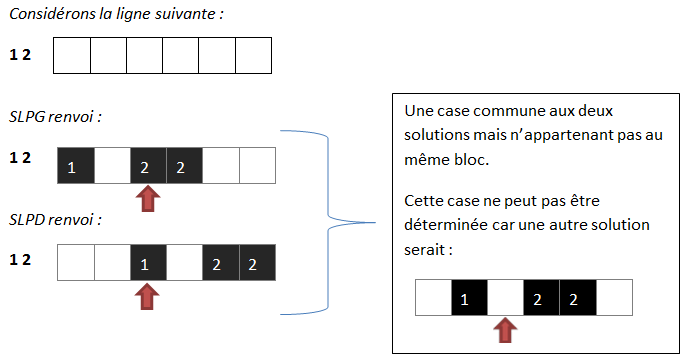
\includegraphics[height=6.5cm,width=12cm]{Exemple1}
\subsubsection{La méthode remplirCasesSureBl}
Cette méthode est appelée après Fusion dans le but de placer les cases blanches sûres. Elle est en mesure de les déterminer grâce aux solutions SLPG-SLPD en calculant les envergures des blocs de cases noires. Dès lors, les espaces situés entre les intervalles trouvés sont des cases blanches sûres.\newline
Elle commence par générer une ligne de cases blanche de la même taille que celles prises en paramétres; à savoir, le résultat de Fusion et les solutions SLPG-SLPD; puis ``noirci'' les cases correspantes à l'intervalle qu'occupe chacun des blocs dans l'une et l'autre des solutions SLPG-SLPD.
\newline
A la fin de ce procédé, elle copie les cases blanches restantes dans le résultat de Fusion.
\subsection{Résolution du Picross}
Pour résoudre un Picross, un appel initial des méthodes précédentes sur toutes les lignes et colonnes est effectuer (cf. TINY\_SOL), cela pour but d'initialiser nos listes d'indices de lignes/colonnes modifiées afin de rappeler les méthodes sur les lignes/colonnes correspondantes, et ce tant que les listes contiennent des cases modifiées (cf. FAT\_SOL).
\subsubsection{la méthode de Backtracking}
A l'aide de nos méthodes précédentes, il peut arriver que des cases ne puissent être déterminées;\newline
Nous avons choisi d'implémenter une méthode de backtracking 'simple' qui place une case indeterminée (arbitrairement, la première qu'il trouve en parcourant les lignes de la matrice) à noire et étudie les conséquences de cette coloration;
L'algorithme est explicité en annexe.
\section{Description de l'implémentation}
\subsection{Les besoins du programme :}
\subsubsection{Pour les indices de chaque ligne/colonne:}
\begin{itemize}
\item Imperatif à satisfaire:
\begin{itemize}
\item structure de taille dynamique (nombre variable d'indices par lignes)
\item parcours en $\theta$(n) (plusieurs méthodes recourant à un parcours total ou partiel de la structure)
\item relation d'ordre (le parcours ne sont réalisés que dans l'ordre de l'indice le plus en haut vers celui le plus en bas respectivement gauche-droite pour les lignes)
\end{itemize}
\item Choix : la liste simplement chainée, car elle correspond parfaitement aux spécifications.
\end{itemize}
\subsubsection{Pour représenter la grille du picross :}
\begin{itemize}
\item Imperatif à satisfaire:
\begin{itemize}
\item structure de taille fixe
\item accès en temps constant a chaque case
\item facilitée de copie de la structure ($\theta$(n))
\end{itemize}
\item Choix: La matrice (Un tableau de tableaux)
\end{itemize}
\subsubsection{Pour l'ensemble des indices de lignes/colonnes :}
\begin{itemize}
\item Imperatif à satisfaire:
\begin{itemize}
\item accès en temps constant a chaque liste
\item indicage cohérent avec la matrice
\end{itemize}
\item Choix : Un tableau de listes
\end{itemize}
\subsubsection{Pour ligmodif/colmodif}
\begin{itemize}
\item Imperatif à satisfaire:
\begin{itemize}
\item ajout d'un élément en temps constant
\item retrait d'un élément en temps constant
\item taille dynamique
\end{itemize}
\item Choix :
Le choix naturel serait l'ensemble mais nous avons choisi la liste simplement chainée car déjà implémentée.
\end{itemize}
\newpage

\subsection{Les classes}
\subsubsection{La classe Cell :}
\begin{itemize}
\item Attributs :
\begin{itemize}
\item Val : contient la valeur d'un bloc de case ou un indice
\item Suiv : pointeur sur la cellule suivante de la liste
\end{itemize}
\end{itemize}
\subsubsection{La classe Liste :}
\begin{itemize}
\item Attributs :
\begin{itemize}
\item Longueur : contient le nombres de cellules de la liste.
\item Fini : indique si la ligne/colonne à laquelle est rattachée la liste est entièrement rempli (booléen à true) ou non (booléen à false), cet attribut est
notamment très utile pour vérifier la condition d'arrêt de notre résolution.
\item Tête : Pointeur vers le premier élément de la liste.
\end{itemize}
\item Méthode remarquable :
\begin{itemize}
\item Surcharge de l'opérateur() : Nous l'utilisons notamment pour faciliter l'accès à un element de la liste.
\end{itemize}
\end{itemize}
\subsubsection{La classe Tabliste :}
\begin{itemize}
\item Attributs :
\begin{itemize}
\item Tab : le tableau de listes
\item Taille : la taille du tableau
\end{itemize}
\item Méthode remarquable :
\begin{itemize}
\item Surcharge de l'opérateur[]: Nous permet l'accès aux listes en temps constant comme pour un tableau.
\end{itemize}
\end{itemize}
\subsubsection{La classe Matrice :}
\begin{itemize}
\item Attributs:
\begin{itemize}
\item Mat : la matrice d'entiers
\item Nbl : Nombre de ligne
\item Nbc : Nombre de colonnes
\end{itemize}
\end{itemize}
\subsection{ La classe Picross :}
La classe picross est la classe dont l'instance représente le picross; S'est dans cette classe que sont implémentées nos méthodes de résolution.
\begin{itemize}
\item Attributs:
\begin{itemize}
\item Une Matrice (-1 : blanc, 0 : indéterminé, 1 : noir)
\item Deux TabListes pour nos listes de blocs
\item Deux listes d'indices ligModif et colModif pour limiter nos récursions
\end{itemize}
\end{itemize}
\subsection{Les algorithmes remarquables :}
\subsubsection{SLG :}
\paragraph{Spécification :}
 void SLG(int*, short int, Cell*, short int, bool\&);
\begin{itemize}
\item Paramètres:
\begin{itemize}
\item Un tableau d'entier: (Donnée/resultat) il représente une ligne/colonne de notre matrice, initialement il peut contenir des cellules à 1,-1,0
\item Un short int : représentant la taille du tableau
\item Une cellule de liste: il repésente le prochain indice a placer dans le tableau, initialement la première cellule associé à la dite ligne/colonne
\item Un short int : représentant l'indice dans le tableau auquel on souhaite placer le bloc, initialement 0
\item Un booléen passé par référence : représentant si il est possible ou non de placer la fin de la liste d'indices indice courant compté a partir de l'indice courant dans le tableau.
\end{itemize}
\item Retour de la fonction.
\end{itemize}
Le retour ce fait par l'intermédiaire du tableau et du booléen. Si le booléen est à false c'est que le couple (ligne/colonne,liste d'indice) n'a pas de solution. Dans le cas contraire, la solution la plus à gauche nous est donnée dans le tableau.
\paragraph{Algorithme : SLG}(L: ligne; n: taille de la ligne; Lind: liste d'indices; i: entier; possible: booleen)
\begin{description}
\item[Debut]
\item[]
  \begin{itemize}
  \item[Si] Lind est vide alors 
    \begin{itemize}
    \item Si L ne contient pas de cases noires après l'indice i alors
      \begin{itemize}
      \item on blanchit toutes les cases de L d'indices supérieurs à i;
      \end{itemize}
    \item Sinon 
      \begin{itemize}
      \item possible == faux;
      \end{itemize}
    \end{itemize}
  \item[Sinon] on essaie de placer le 1er bloc de Lind à l'indice i
    \begin{itemize}
    \item Si on y arrive pas alors
      \begin{itemize}
      \item si L[i] n'est pas noir alors 
        \begin{itemize}
        \item SLG(L, n, Lind, i+1, possible);
        \end{itemize}
      \item sinon 
        \begin{itemize}
        \item possible == faux;
        \end{itemize}
      \end{itemize}
    \item Sinon
      \begin{itemize}
      \item SLG(L, n, queue(L), i+tête(L)+1, possible);
      \end{itemize}
    \end{itemize}
  \item[Si] non possible alors 
    \begin{itemize}
    \item Si L[i] n'est pas noir alors
      \begin{itemize}
      \item SLG(L, n, Lind, i+1, possible);
      \end{itemize}
    \item Sinon 
      \begin{itemize}
      \item possible == faux;
      \end{itemize}
    \end{itemize}
  \end{itemize}
\item[Fin algorithme]
\end{description}
\paragraph{Complexité pire des cas : $\theta(n^2) <$c$\leq\theta(2^n)$\\ }
 Notons :
\begin{itemize}
\item i: l'indice dans notre tableau
\item n: la taille du dit tableau
\item T: le dit tableau
\item l: la taille de la liste d'indice (le nombre d'indices)
\item $m_i$: l'envergure d'un indice i
\end{itemize}
Dans le pire des cas de notre algorithme, on peut imaginer que chaque hypothèse faite par notre algorithme soit fausse. Pour cela, il nous faut imaginer une liste d'indice de petite taille (ici on choisira $\forall$i $\in$[0,l[ $m_i$=1). En effet, plus les indices sont grands moins ils ont de positions possibles pour une même taille de tableau, et donc moins d'hypothèses.
\newline Enfin, on voit bien que la complexité va dépendre de la taille de la liste; en effet, chaque cellule appelle la fonction au moins une fois pour chaque maillons placé après dans liste. Au plus, pour un indice j de la liste SLG sera appeé $\sum_{i=l-j}^{l} (i)$ fois c'est à dire l-i fois $\forall$i $\in$[j,l[.
\newline En outre, on sait que le coût de SLG sans les appels récursifs revient à n puisque dans tous les cas où la liste n'est pas vide, on recopie le tableau. Sinon, si la liste est vide, on parcours le tableau de l'indice i à n. Ici, on considérera cette valeur cst=n, bien que ce cas soit défavorable. Il n'est pas réaliste en effet, dans le cas d'une liste non-vide (ce qui est notre cas) cette valeur est nécessairement inférieure et decroit tout au long des appels de SLG.
Soit une complexité inférieure à $2^n$.
\newline
Avec ce modèle défavorable on obtient l'équation de recursion suivante:
\begin{center}
 \fbox{SLG(i)= $\sum_{k=l-i}^{l} (SLG(k)*n)+cst$}
\end{center}
Ainsi, en notant c la complexité dans ce pire des cas: $\theta(n^2) <$c$\leq\theta(2^n)$; pour chaque case on parcours au minimun une fois le tableau (la recopie) pour chaque cellule après ici cela fait déjà $\theta(n^2)$ et on doit le faire pour chaque indice.
\paragraph{Complexité meilleur des cas : $\theta$(n)\newline}
Dans le meilleur des cas la liste est vide, on doit pacourir une fois le tableau pour pouvoir vérifier.
\subsubsection{remplirCasesSureBl :}
\paragraph{Spécification :}remplirCasesSureBl(int* Merge, int* TG,int* TD, sint taille, Liste \&L);
\begin{itemize}
\item Paramètres:
\begin{itemize}
\item Un tableau d'entier Merge: (Resultat) il représente la ligne/colonne de la matrice,après la résolution de notre fonction, initialisé avec le retour de fusion.
\item Un tableau d'entier TG: (Donnée) il représente la solution la plus à gauche qui résout notre ligne/colonne en fonction de sa liste d'indices et des informations à notre disposition
\item Un tableau d'entier TD: (Donnée) idem pour la solution la plus à droite
\item Un short int taille: représentant la taille du tableau
\item Une liste d'indices L: La liste d'indices associés a la ligne/colonne
\end{itemize}
\item Retour de la fonction:
\end{itemize}
La fonction retourne par l'intermédiaire du tableau Merge notre ligne/colonne de depart avec en plus d'éventuelles case blanches "sures" en se basant sur l'envergure des blocs.
\paragraph{Comlexité : $\theta(n)$\newline}
On doit pour chaque indice de la liste inscrire son envergure dans un tableau intermediaire, pour cela il nous faut parcourir SLG puis SLD mais pas en totalité, en effet, on parcours SLG jusqu'a trouver un indice i1 tel que TG[i1]=0.
On continu notre parcours jusqu'a trouver un indice i2 tel que TG[i2]=0, c'est alors qu'on parcours SLD à partir de i2-1 jusqu'a trouver un indice i3 tel que TG[i3]=0. 
On a alors l'envergure du premier bloc. Pour le deuxiéme on peut commencer notre parcours dans SLG à partir de i2 car il est forcément à droite du premier.\newline 
On trouve alors un nouveau i1 puis un i2 puis un i3 et on recommence alors à partir du nouveau i2 et ainsi de suite. Au final, on aura parcouru entre n et 2n case du tableau.
\subsubsection{Backtrack :}
\paragraph{Spécification :}
 void backtrack(bool \&poss);
\begin{itemize}
\item Param\`etre:
\begin{itemize}
\item Un booléen signalant la possibilité de placer une case dans un picross non fini
\end{itemize}
Dans le cas ou cela est possible, on "backtrack" une case
Dans le cas ou cela n'est pas possible, on revient à l'environnement de la dernière case backtrackée et on l'inverse
\item Retour de la fonction :
\end{itemize}
La fonction ne retourne rien, on travaille directement sur notre Matrice.\newline
Cela à pour conséquence une complexité élevée ($\theta(n^2)$) lors de la recopie de celle-ci.
\subsection{ L'interface graphique:}
Pour implémenter une interface utilisateur graphique et afficher notre Picross on utilise la bibliothèque Gtkmm, qui est une surcouche de GTK pour le langage C++.
Dans une fenêtre du programme on a quatre boutons:
\begin{itemize}
\item  ``Description'' contient une brève description du programme;
\item ``Ouvrir'' pour ouvrir un fichier texte (nos grilles Picross), qui permet l'initialisation d'une grille vide avec ses indices;
\item ``Résolution'' permet le déclenchement de nos méthodes de résolution et affiche la grille ainsi résolue;
\item ``Quitter'' appel d'une fonction GTK permettant la fermeture de la fenêtre.
\end{itemize}
\begin{landscape}
\begin{figure}
\begin{center}

\includegraphics[width=15cm]{picross}
\end{center}
\caption{Un exemple de solution Picross.}
\end{figure}
\end{landscape}
\section{Ameliorations/Evolution du programme:}
\begin{itemize}
\item Dans le cas ou le picross nécessite un backtrack pour sa résolution, les blocs restants peuvent se voir attribuer un degré de liberté, et la case ainsi determinée la plus probable aurait alors été celle choisi pour lancer le backtracking.
\item Dans le souci d'améliorer la compléxitée de la résolution d'une grille en moyenne, nous aurions pû, plutôt que de faire des copies/recopies de matrices entre les environnements de backtrack, ne maintenir que les cases modifiées entre les environnements de backtracks;
Cela dit, dans le pire des cas (aucune case n'est determinable), la complexité reste équivalente ($theta(n^2)$) car l'ensemble des cases se verraient modifiées après le premier environnement de backtrack. (Exemple BT 1 sol)
\item Nous aurions pû implémenter des methodes permettant de rentrer des grilles de picross graphiquement (au clic).
\item Dans certains cas la méthode pour trouver les cases blanches sûres que nous avons choisies ne trouve pas toutes les cases blanches que nous aurions pu déterminer. Par exemple :
\begin{center}
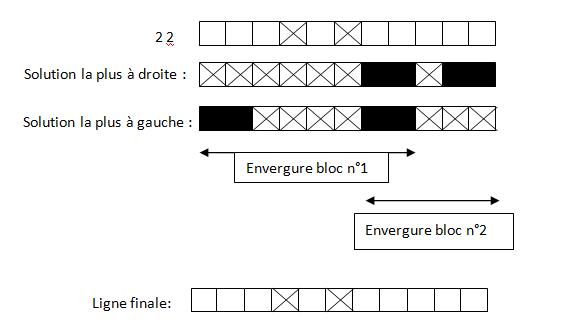
\includegraphics[width=11cm]{image1}
\end{center}
En effet, il n’y a aucun chevauchement de noir appartenant au même bloc, et aucun blanc qui ne soit dans l’envergure des blocs. Pourtant on peut aisément voir que la case d’indice 4 (indice débutant à 0) est blanche puisqu’elle est coincée entre deux blanches et que la taille minimum des blocs est de deux. On pourrait donc imaginer un algorithme qui teste pour chaque bloc d’indéterminé coincé entre deux blancs si sa taille est inferieure au plus petit indice à rentrer,  dans ce cas on le blanchit. Néanmoins, on pourrait imaginer un algorithme plus fin. Regardons cet autre exemple :
\begin{center}
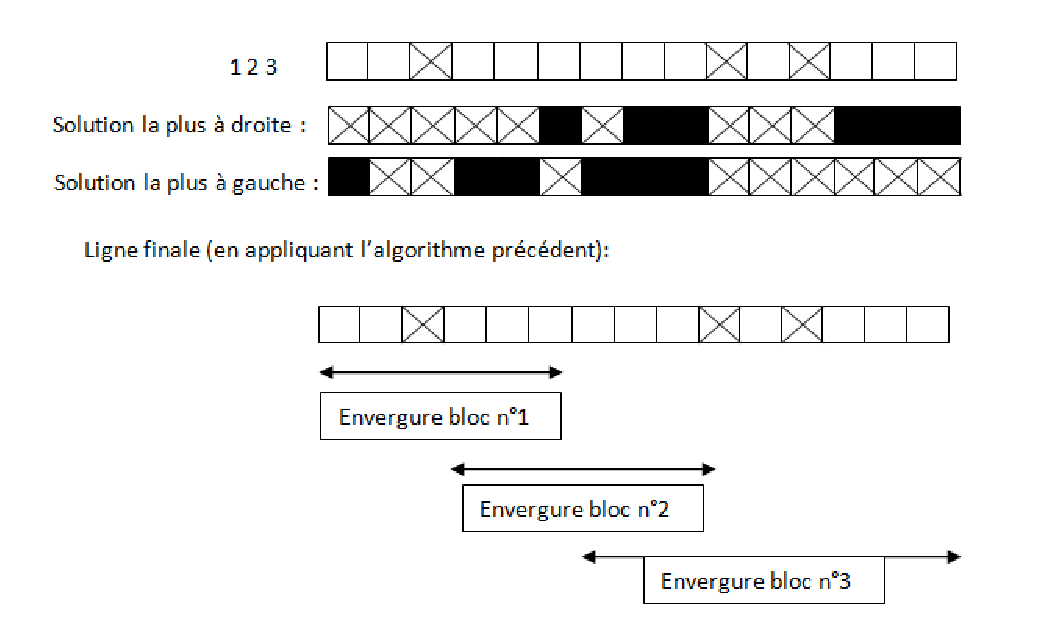
\includegraphics[width=11cm]{image2}
\end{center}
Ici on voit bien que la cellule 11 devrait être blanche puisque qu’elle n’est pas dans l’envergure du seul bloc qui pourrait convenir. Ainsi, en sachant que la solution la plus à gauche générale et la solution la plus à droite générale définissent aussi respectivement la solution la plus à droite et la solution la plus à gauche de chaque bloc, on aurait pu définir un algorithme qui, en fonction de ces deux solution et de la liste d’indices, vérifie pour chaque bloc d’indéterminé coincé entre deux blanc (ou un bord) s’il est dans l’envergure des indices qui sont inférieurs à sa taille.
\end{itemize}
\section{Annexes :}
\subsection{Schéma de l'implémentation : }
\begin{landscape}
\begin{figure}
\begin{center}
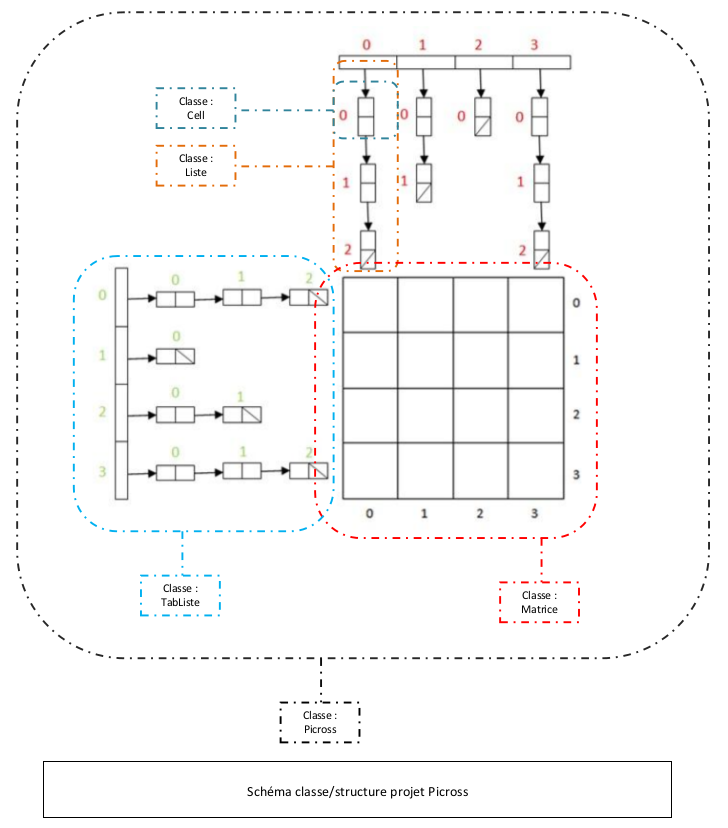
\includegraphics[width=14cm]{./images/recapitulatif_stucture.png}
\end{center}
\end{figure}
\end{landscape}
\newpage
\subsection{Lecture d'un fichier pour construire une grille:}
Dans le but de construire une grille Picross nous avons choisi du structurer un fichier texte de la manière suivante :\newline
Les deux premiers nombres séparés d'un espaces représentent nos Lignes | Colonnes.
La méthode passe ensuite sur toutes les lignes du fichier, ou chaque saut de ligne correspond à une nouvelle liste de tabListe.
\begin{figure}[h]
\begin{center}
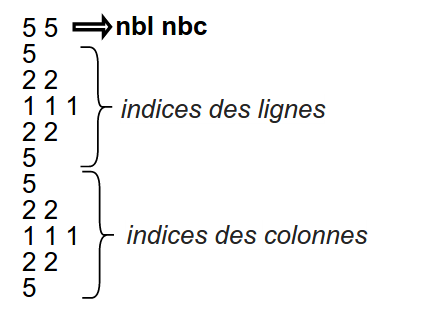
\includegraphics[width=8cm]{ex2}
\end{center}
\caption{Un exemple de fichier.}
\end{figure}
\newpage
\subsection{Algorithme SLG :}
\begin{verbatim}
void Picross::SLG(int* Tab, size_t n, Cell* P, size_t i, bool &poss)
{
  if(P && i<n)
  {
    int* Tab2=new int [n];
    for(size_t j=0;j<n;j++)
    {
      Tab2[j]=Tab[j];
    }
    PlacerBloc(Tab,n,P->getVal(),i,poss);
    if(poss)//si j'ai placer mon bloc
    {
      SLG(Tab,n,P->getSuiv(),i+P->getVal()+1,poss);//bloc suivant
      if(!poss)
      {
        for(size_t j=0;j<n;j++)
        {
          Tab[j]=Tab2[j];
        }
	      if(Tab[i]==1){poss=false;}
        else{SLG(Tab,n,P,i+1,poss);}
      }
    }
    else
    {
      if(Tab[i]==1){poss=false;}
      else{SLG(Tab,n,P,i+1,poss);}
    }
    delete [] Tab2;
  }
  else
  {
    poss=Verification(Tab,i,n);
    if(poss)
    {
	    for(size_t i=0; i<n; i++){if(Tab[i]==0){Tab[i]=-1;}}
    }
  }
}
\end{verbatim}
\newpage
\subsection{Algorithme de backtracking :}
\begin{verbatim}
void Picross::backtrack(bool &poss)
{
  FAT\_SOL(ligModif.getLongueur()); //méthode de résolution
  if(!isPicrossFini())
  {
    int** SAVE=copieMat();	//Copie de la matrice
    bool* TL=new bool [getNbLignes()];
    bool* TC=new bool [getNbColonnes()];
    copieBool(TL,TC);	//Copie de nos booléens lignes|colonnes finies
    sint i=0,j=0;	//Indices utilisés pour le placement de la case noire
    Placer1noir(poss,i,j);	//poss à true ssi la matrice contient un indeterminé(0) qu'on à pu mettre à noir(1)
    if(poss)
    {
      backtrack(poss);	//On recommence
	//Si, a la suite des appels recursifs, le picross n'est pas correctement rempli et on ne peut pas Placer1noir:
	//A ce niveau nous sommes dans le dernier environnement où on à Placer1noir en (i,j)
      if(!poss)
      {
        recopieMat(SAVE);	//Recopie de la matrice sauvegardée avant le placement du noir
        recopieBool(TL,TC);	//Recopie de nos booléens de lignes|colonnes finies qui aurait pu être modifiés par FAT_SOL de l'environnement précédent
        Placer1blanc(i,j);	//On place la case (i,j) à blanc, car on est sûr qu'elle n'est pas noire
        backtrack(poss);	//On recommence
      }
    }
  }
}
\end{verbatim}
\end{document}
